\begin{problem}[Primer ejemplo elíptico]

Antes de modificar el programa~\ref{code:elliptic1D.m}, responda las
siguientes preguntas.

\begin{enumerate}
    \item

          ¿Cuál ecuación diferencial se está resolviendo?

          \begin{solution}
              Se está resolviendo la ecuación de Poisson con el
              problema de valor de frontera Robin~\cite{CORBINO2020112326}
              \begin{equation}\label{eq:poisson1drobindconditions}
                  \left\{
                  \begin{aligned}
                      \diff[2]{u}{x}
                       & =e^{x},
                      \text{ para }x\in\left[0,1\right].     \\
                      0
                       & = u\left(0\right)-\diff{u}{x}[x=0]. \\
                      2e
                       & =u\left(1\right)+\diff{u}{x}[x=1].  \\
                  \end{aligned}
                  \right.
              \end{equation}
          \end{solution}

    \item

          ¿Cuál es la función de fuerza o lado derecho?

          \begin{solution}
              La función de fuerza es $f=e^{x}$.
          \end{solution}

    \item

          ¿Cuál es el tipo de condiciones de contorno y cuáles son
          los valores de su lado derecho?

          \begin{solution}
              El tipo de condición de contorno es Robin con dos
              coeficientes iguales a $1$.
              El lado derecho es $g_{x=0}=0$ y $g_{x=1}=2e$.
          \end{solution}

    \item

          ¿Cuál es la solución exacta?

          \begin{solution}
              Integramos dos veces y obtenemos la solución general.
              \begin{align*}
                  \iint
                  \diff[2]{u}{x}
                  \dl x           & =
                  \iint
                  e^{x}
                  \dl x.              \\
                  \int
                  \diff{u}{x}
                  \dl x           & =
                  \int
                  \left(e^{x}+C_{1}\right)
                  \dl x.              \\
                  u\left(x\right) & =
                  e^{x}+C_{1}x+C_{2}.
              \end{align*}
              Ahora, apliquemos las condiciones de frontera Robin.
              \begin{equation}\label{eq:linearsystem}
                  \left\{
                  \begin{aligned}
                      0
                       & =
                      u\left(0\right)-
                      \diff{u}{x}[x=0]=
                      e^{0}+C_{1}\left(0\right)+C_{2}-
                      \left(e^{0}+C_{1}\left(1\right)\right)=
                      C_{2}-C_{1}. \\
                      2e
                       & =
                      u\left(1\right)+
                      \diff{u}{x}[x=1]=
                      e^{1}+C_{1}\left(1\right)+C_{2}+
                      \left(e^{1}+C_{1}\right)=
                      2e+2C_{1}+C_{2}.
                  \end{aligned}
                  \right.
              \end{equation}
              El sistema~\eqref{eq:linearsystem} tiene como solución
              $C_{1}=C_{2}=0$.
              Así, la solución exacta
              de~\eqref{eq:poisson1drobindconditions} es
              $u\left(x\right)=e^{x}$.
          \end{solution}
\end{enumerate}

\textsf{\bfseries Explicación del programa}

En la línea $1$ encontramos el
\emph{shebang}\footnote{\url{https://en.wikipedia.org/wiki/Shebang_(Unix)}},
esto permite ejecutar un script de Octave \mintinline{bash}|./elliptic1D.m|
con la opción de modo de procesamiento por lotes (batch), para esto
se necesita tener permisos de ejecución (por ejemplo,
\mintinline{bash}|chmod +x elliptic1D.m|).

\begin{listing}[ht!]
    \tiny
    \centering
    \inputminted{text}{octave-help.txt}
    \caption{\href{https://raw.githubusercontent.com/carlosal1015/mole_examples/refs/heads/main/homework/octave-help.txt}{\mintinline{text}|octave-help.txt|}
        muestra la lista de opciones de Octave por la línea de comandos.}
\end{listing}

En las líneas $2$ al $10$ tenemos un comentario sobre el programa de modo que
ayude al codificador a obtener un contexto del problema a resolver.

% En la línea $4$, la función
% \href{https://docs.octave.org/latest/Cursor-Motion.html#index-clc}{\mintinline{octave}|clc|}
% limpia la pantalla del terminal y mueve el cursor a la esquina superior izquierda.

% En la línea $5$, la función
% \href{https://docs.octave.org/latest/Manipulation-of-Plot-Windows.html#index-close-3}{\mintinline{octave}|close all|}
% cierra todas las ventanas de las figuras con manejadores visibles.

En la línea $12$, la función
\href{https://docs.octave.org/v9.3.0/Manipulating-the-Load-Path.html#index-addpath}{\mintinline{octave}|addpath|}
agrega el directorio \mintinline{octave}|"/usr/share/mole/matlab/"| a la ruta de búsqueda de la función.
Allí se encuentra el directorio de la biblioteca MOLE.

\begin{listing}[ht!]
    \tiny
    \centering
    \inputminted{text}{moledirectoriesoctave.txt}
    \inputminted{text}{moledirectoriescpp.txt}
    \caption{\href{https://raw.githubusercontent.com/carlosal1015/mole_examples/refs/heads/main/homework/moledirectoriesoctave.txt}{\mintinline{text}|moledirectoriesoctave.txt|}
        y \href{https://raw.githubusercontent.com/carlosal1015/mole_examples/refs/heads/main/homework/moledirectoriescpp.txt}{\mintinline{text}|moledirectoriescpp.txt|}
        muestran la estructura de árbol de directorios de la biblioteca MOLE.}
\end{listing}

En las líneas $14$ y $15$, se inicializan los identicadores
\mintinline{octave}|west| (oeste, izquierda),
\mintinline{octave}|east| (este, derecha) con los valores de $0$ y
$1$, respectivamente, estos representan los valores de frontera del
dominio espacial en~\eqref{eq:poisson1drobindconditions}.

En la línea $21$, llamamos a la función
\href{https://carlosal1015.github.io/mole_examples/api_docs/matlab/src/matlab/lap.html}{\mintinline{octave}|lap|},
este genera un operador Laplaciano discreto extendido que requiere
como argumentos obligatorios el orden de precisión
\mintinline{octave}|k|, el número  de celdas \mintinline{octave}|m|
y el tamaño de paso \mintinline{octave}|dx|.
\begin{equation*}
    L=L^{\left(k\right)}=
    D^{\left(k\right)}
    G^{\left(k\right)}=
    DG.\qquad\qquad
    \left(
    \difc.L.{}{}=\nabla\cdot\nabla
    \right),
\end{equation*}
donde $D$ y $G$ son los operadores miméticos de divergencia y gradiente, respectivamente.
Dado que $D\in\mathbb{R}^{\left(m+2\right)\times\left(m+1\right)}$
y $G\in\mathbb{R}^{\left(m+1\right)\times\left(m+2\right)}$, entonces $L\in\mathbb{R}^{\left(m+2\right)\times\left(m+2\right)}$.

En la línea $22$, con la función \href{https://docs.octave.org/v9.3.0/Figure-Properties.html#index-figure-visible}{\mintinline{octave}|figure|}
desactivamos que se muestre la figura en la pantalla, preferimos solamente guardar la gráfica.

En la línea $23$, con la función \href{https://docs.octave.org/latest/Information.html#index-spy}{\mintinline{octave}|spy|}
graficamos (no se mostrará) el patrón de dispersidad de $L$.

En la línea $24$, con la función \href{https://docs.octave.org/latest/Printing-and-Saving-Plots.html}{\mintinline{octave}|saveas|}
guardamos esta gráfica en formato PDF y recortado.

En la línea $29$, llamamos a la función
\href{https://carlosal1015.github.io/mole_examples/api_docs/matlab/src/matlab/robinBC.html}{\mintinline{octave}|robinBC|},
este requiere como argumentos obligatorios el orden de precisión \mintinline{octave}|k|,
el número  de celdas \mintinline{octave}|m|, el tamaño de paso
\mintinline{octave}|dx|, el coeficiente Dirichlet \mintinline{octave}|a| y el coeficiente Neumann \mintinline{octave}|b|.
Esta función devuelve una matriz en $\mathbb{R}^{\left(m+2\right)\times\left(m+2\right)}$.

\begin{algorithm}[H]
    $A\leftarrow L$\;
    $u\leftarrow g$\;
    $A\leftarrow A+R_{G}$\;
\end{algorithm}

\href{https://docs.octave.org/latest/Exponents-and-Logarithms.html#XREFexp}{\mintinline{octave}|exp|}

\begin{listing}[ht!]
    \tiny
    \centering
    \inputminted[frame=single,framesep=10pt,linenos,firstline=1,lastline=51,highlightlines={21,29}]{octave}{../examples/octave/elliptic1D.m}
    \caption{Programa~\texttt{elliptic1D.m}}
    \label{code:elliptic1D.m}
\end{listing}

\begin{listing}[ht!]
    \tiny
    \centering
    \inputminted[frame=single,framesep=10pt,linenos,firstline=1,lastline=63,highlightlines={23,26}]{cpp}{../examples/cpp/elliptic1D.cpp}
    \caption{Programa~\texttt{elliptic1D.cpp}}
\end{listing}

\begin{listing}[ht!]
    \tiny
    \centering
    \inputminted[firstline=1,lastline=8,highlightlines={7}]{cmake}{../examples/cpp/CMakeLists.txt}
    \inputminted[firstline=14,lastline=14]{cmake}{../examples/cpp/CMakeLists.txt}
    \inputminted[firstline=16,lastline=16,highlightlines={16}]{cmake}{../examples/cpp/CMakeLists.txt}
    \inputminted[firstline=65,lastline=69]{cmake}{../examples/cpp/CMakeLists.txt}
    \caption{Programa~\texttt{CMakeLists.txt}}
\end{listing}

\begin{itemize}
    \item

          \url{https://arma.sourceforge.net/docs.html#Col}.

    \item

          \url{https://docs.octave.org/v9.3.0/Creating-Sparse-Matrices.html}

    \item

          \url{https://docs.octave.org/v9.3.0/Information.html}

    \item

          \url{https://www.mathworks.com/matlabcentral/fileexchange/44354-curvilinear-2d-grid-poisson}
\end{itemize}

\begin{figure}[ht!]
    \centering
    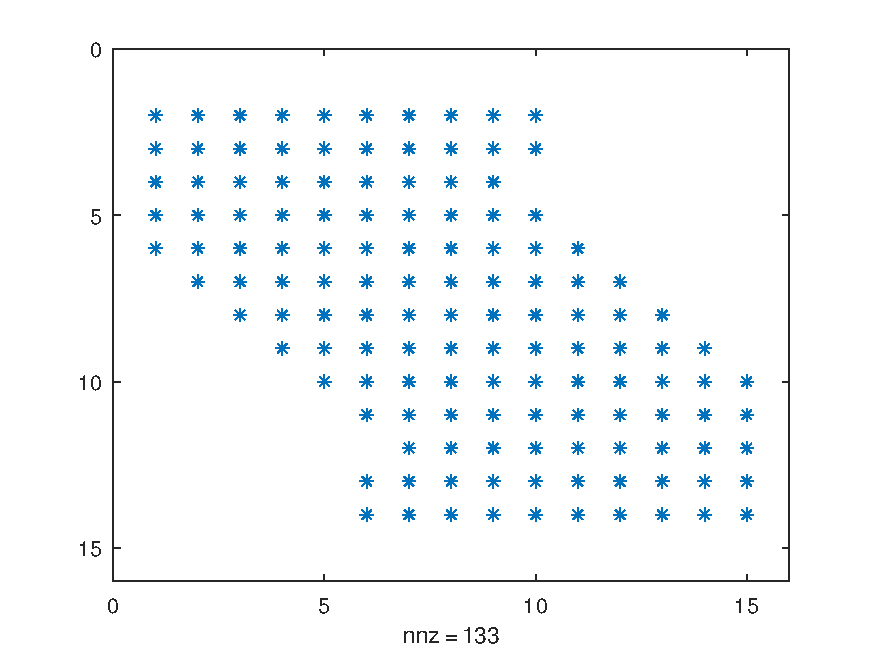
\includegraphics[width=.39\paperwidth]{../examples/octave/elliptic1Dsparsebefore.pdf}
    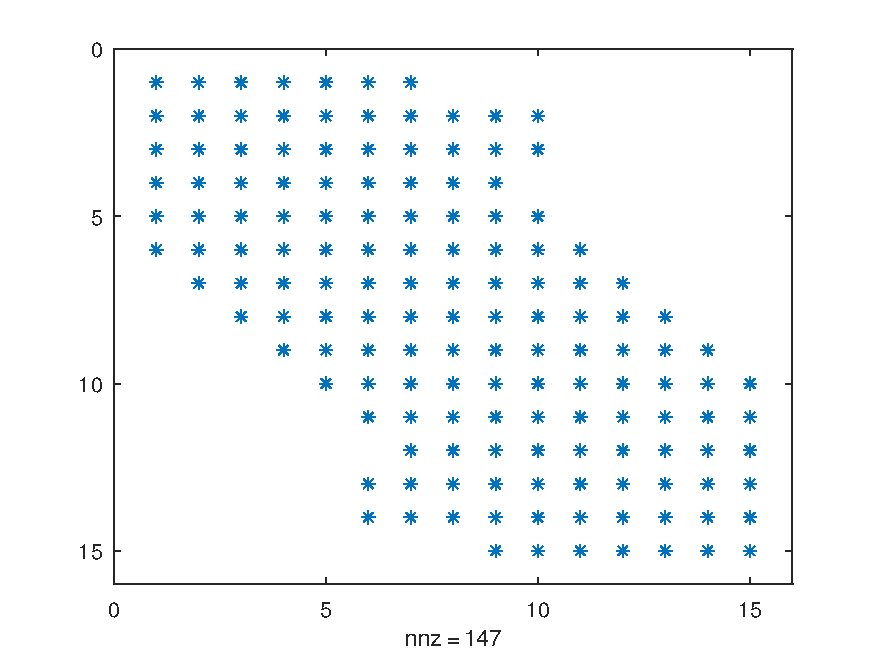
\includegraphics[width=.39\paperwidth]{../examples/octave/elliptic1Dsparseafter.pdf}
    \caption{Izquierda: Representación dispersa de $L$ hasta la línea 13.
        La primera fila y última fila son vectores nulos.
        Derecha: Representación dispersa de $L$ hasta la línea 21.
        La matriz $L\in\mathbb{R}^{15\times 15}$.}
\end{figure}

\begin{figure}[ht!]
    \centering
    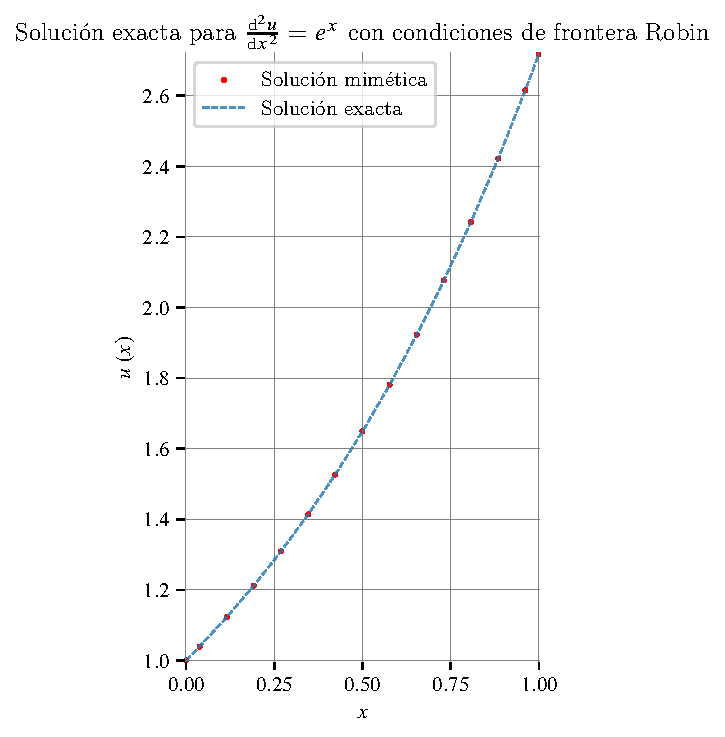
\includegraphics[width=.39\paperwidth]{elliptic1D.pdf}
    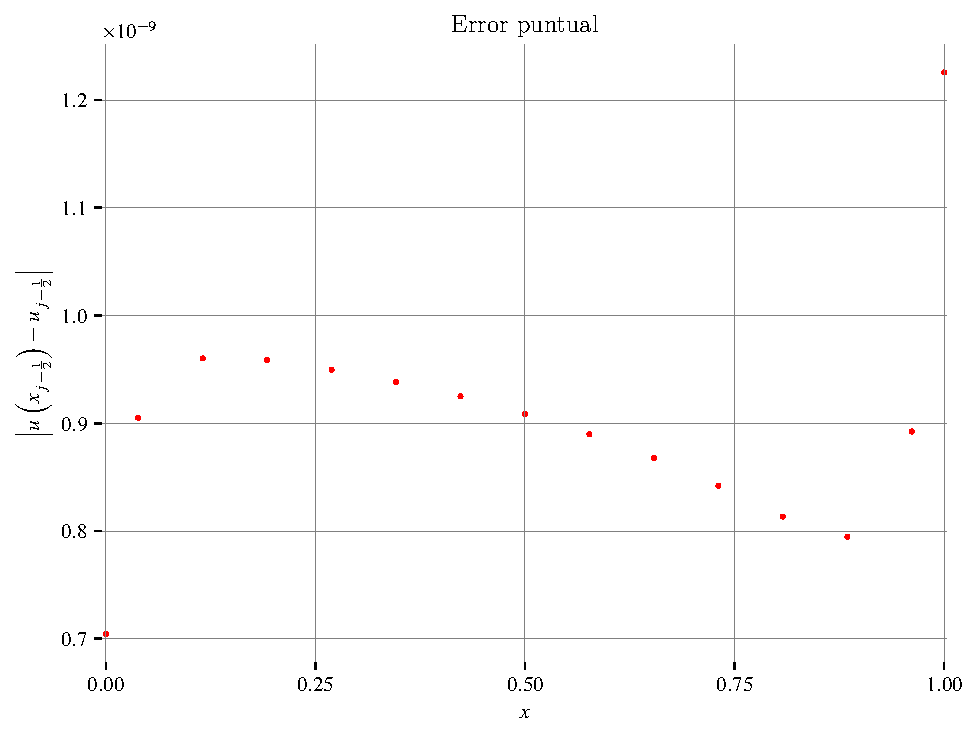
\includegraphics[width=.39\paperwidth]{elliptic1Derror.pdf}
    \caption{Izquierda: Antes. Derecha: Después.}
\end{figure}

\begin{figure}[ht!]
    \centering
    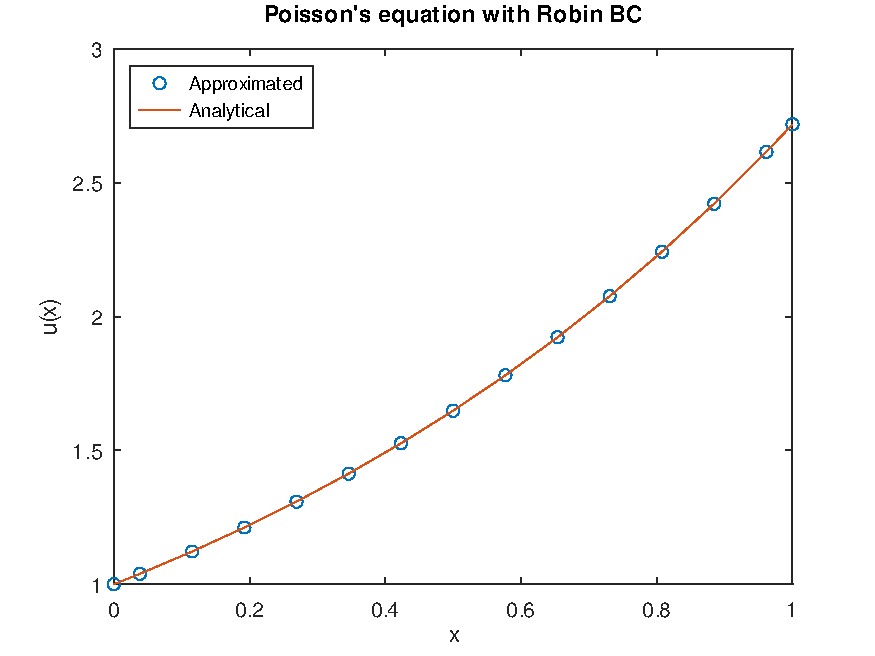
\includegraphics[width=.6\paperwidth]{../examples/octave/elliptic1D.pdf}
    \caption{Solución al problema usando \mintinline{octave}|k=6| y \mintinline{octave}|m=2k+1=13|.}
\end{figure}

\noQED % Use \noqed or \noQED at the end to suppress the Q.E.D. symbol that marks the end of the current problem.
\end{problem}

\begin{problem}
.
\end{problem}

\begin{solution}
    % You may write claims, lemmas, propositions, etc. inside your solution.
    \begin{lemma}\label{lem}
        Some auxiliary result.
    \end{lemma}
    \begin{proof}
        The proof of \cref{lem}, where we use the following formula:
        \[
            \infty = \infty + 1.
            \qedhere % For placing the Q.E.D. symbol in the right place.
        \]
    \end{proof}
    \begin{fact}[This statement requires no proof]
        \proofless % To change the hollow box marking the end of a theorem-type environment into a solid one.
        Some statement.
    \end{fact}
    ... and the rest steps...

\end{solution}